%% Section to describe and comment the results from the experiments performed.
%% lang: en-GB

In this section, we detail the accomplished experiments and their results. In 
order to evaluate properly the project's timing requirements, we have performed 
three experiments:

\begin{itemize}
	\item \textbf{A WR node comparison:} We have compared the three WR devices 
	analysed previously. The PPS stability is measured.
	\item \textbf{A scalability test:} The second experiment covers a 
	scalability analysis of the WR solution for the SKA timing system. We 
	looked to determine if WR is able to fully synchronize the entire number of 
	nodes expected in the SKA telescope.
	\item \textbf{A test under changing environmental conditions:} We measure 
	the PPS stability while changing the external conditions for the fibre 
	link, as it is expected in the final deployment.
\end{itemize}

The principal equipment and tools utilized during the experiments are listed 
below:

\begin{itemize}
    \item Two \textbf{WRS} to emulate a two-hops WR network. Both are 
    hardware version 3.4 and are flashed with the last version of the WR 
    firmware (v5.0).
    
    \item A \textbf{WR-LEN} (hardware v1.0) an a \textbf{SPEC} board with a FMC 
    DIO connected for the comparison between WR nodes.
    
    \item Two \textbf{WR-ZEN TP} (Time Provider) to test the 
    performance of the new developed platform as WR nodes of the SKA 
    facilities. Firmware version is 1.2 while the hardware is v3.0.
    
    \item A High-resolution counter from \textbf{Keysight}, the \textbf{52320A}.
    
    \item Multiple components for the setup of the equipment:
    \begin{itemize}
        \item Small form-factor pluggable transceptors (SFPs) to establish the 
        link between WR devices. For the shorter links we have used the most 
        common bidirectional SFPs for WR: AXCEN 1310/1490 nm. For larger links, 
        we tried 
        SFPs from FiberStore: GE-BX-80 1490/1550 nm.
        \item Simplex optical fibre links (G652D). For the device 
        characterization short distance fibres have been used, meanwhile for 
        the scalability and temperature tests we have used long distance links: 
        20 and 50 km respectively.
        \item An OCXO Morion MV89 as frequency reference for the GM mode.
    \end{itemize}
    
\end{itemize}

\subsection{PPS performance}
\label{subsec:pps_performance}

The PPS performance is evaluated for the three WR nodes analysed previously. 
Each node, was connected to the same WRS with a short fibre link (Figure 
\ref{fig:prueba1pps}). Once the node was fully synchronized, we started to 
measure the time interval between the PPS from the WRS and the PPS from the 
slave node. All measurements last 24 hours under laboratory conditions.

\begin{figure}[H]
	\centering
	\includegraphics[width=0.7\linewidth]{img/prueba1_pps}
	\caption[Connection diagram for the PPS performance test.]{For the PPS 
	performance test, the PPS output of the device under test (DUT) is input to 
	a timer that measures the time interval between the PPS from the WRS and 
	the PPS from the DUT.}
	\label{fig:prueba1pps}
\end{figure}

Figure \ref{fig:tdev_exp1} corresponds to the Time Deviation (TDEV) statistic. 
It express the stability of the phase difference between the WR master and the 
WR slave versus the observation interval, $\tau$. For a $\tau=1$ we obtained a 
TDEV value of 1.47e-11 for the WR-ZEN. This is 3.6e-12 s and 1.18e-11 s less than WR-LEN and SPEC, respectively. The lowest value is 1.0e-12 s for the WR-ZEN. Differences between the lowest values of WR-LEN and the SPEC board respect to the WR-ZEN are: 6.2e-13 and 4.6e-13 respectively.

\begin{figure}
    \centering
    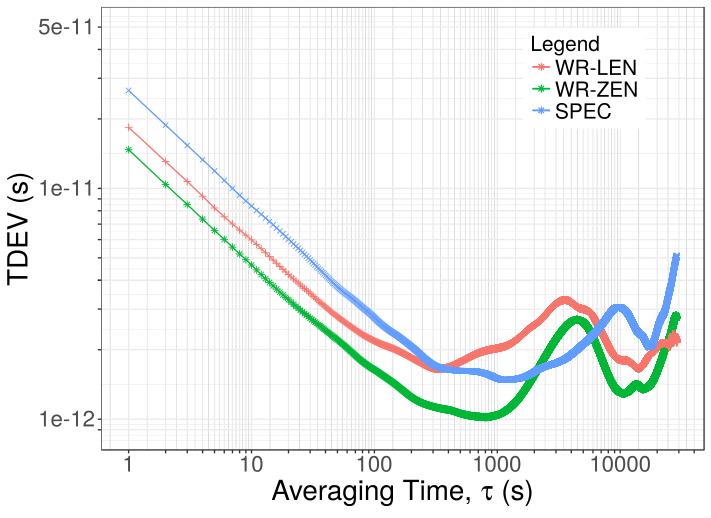
\includegraphics[width=0.7\linewidth]{img/tdev_exp1}
    \caption[TDEV for the WR devices comparison.]{The Time Deviation plot show 
        that all devices maintain good PPS performance. Nevertheless, the 
        WR-ZEN 
        achieves the best results.}
    \label{fig:tdev_exp1}
\end{figure}

Modified Allan Deviation (MDEV) results are included in Figure 
\ref{fig:mdev_exp1}. From the TDEV (\ref{fig:tdev_exp1}) and MDEV (\ref{fig:mdev_exp1}) results we observe that white PM noise dominates from $\tau=1$ to a few hundred os seconds averaging time (depending of the observed device). After that, the rest remains as flicker FM noise.

\begin{figure}
    \centering
    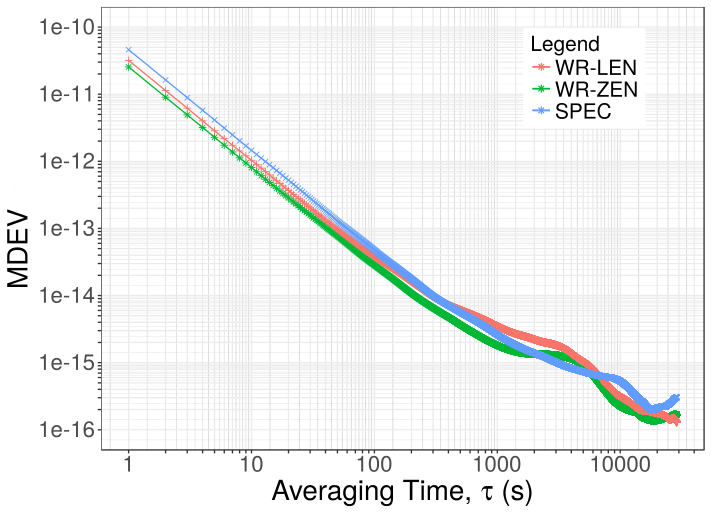
\includegraphics[width=0.7\linewidth]{img/mdev_exp1}
    \caption[MDEV for the WR devices comparison.]{The Modified Allan Deviation 
        plot show there is not undesired noise effects on any of the three 
        devices. 
        In the three plots the dominant noise is phase modulated white noise.}
    \label{fig:mdev_exp1}
\end{figure}

%\begin{table*}\centering
%	\ra{0.8}
%	\begin{tabular}{@{} cccccccccccc@{}}%\toprule
%		& \multicolumn{3}{c}{\bfseries{SPEC}} &&
%		\multicolumn{3}{c}{\bfseries{WR-LEN}} && 
%		\multicolumn{3}{c}{\bfseries{WR-ZEN}} \\
%		\cmidrule(l){2-5}  \cmidrule{6-9} \cmidrule{10-12}
%%		\small{\textbf{$\tau$ (s)} & MDEV & TDEV & MTIE & & MDEV & TDEV & MTIE 	
%%		& & MDEV & TDEV & MTIE} \\
%		\small{\textbf{$\tau$ (s)}} & \tiny{MDEV} & \tiny{TDEV} & 
%		\tiny{MTIE} & & \tiny{MDEV} & \tiny{TDEV} & 
%		\tiny{MTIE} & & \tiny{MDEV} & \tiny{TDEV} & 
%		\tiny{MTIE} \\
%		1 & X & Y & Z && 
%		\bottomrule
%	\end{tabular}
%	\caption{In this table it can be checked out the most relevant statistics 
%	for the device characterization performed in the subsection \ref{subsec: 
%	charact_zen}. \textcolor{red}{esto hay que explicarlo más e intentarlo 
%	meterlo dentro de su sección}}
%	\label{tab:exp1res}
%\end{table*}

Finally worst case analysis is done with the Maximum Time Interval Error (MTIE) 
statistic (Figure \ref{fig:mtie_exp1}). With the TDEV results, we observed that 
all the WR devices fulfil the 2 ns time budget requirement. In the worst case, 
we also observed that requirement is well fulfilled. For the WR-ZEN the 
difference between the WRS PPS and its PPS is bounded on 1.5e-10 s. Again, the 
WR-ZEN achieves the best results: 3.90e-11 less than the WR-LEN and Y less that 
SPEC.

\begin{figure}
	\centering
	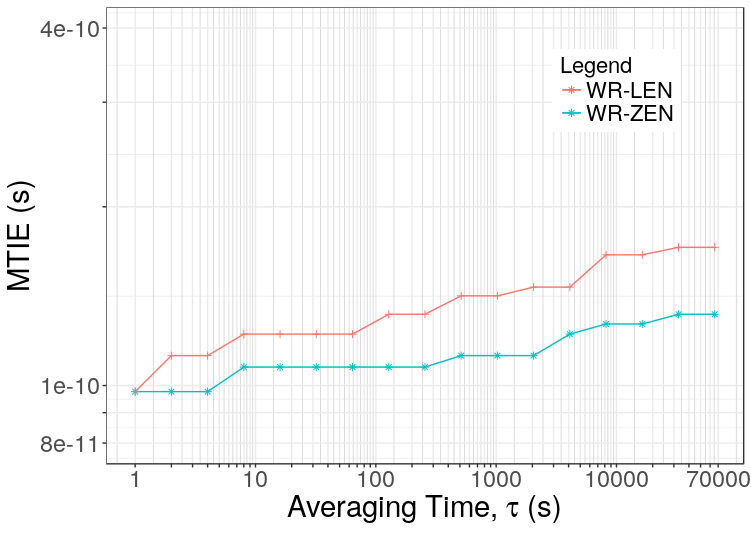
\includegraphics[width=0.7\linewidth]{img/mtie_exp1}
	\caption[MTIE for the WR devices comparison.]{The worst case scenario 
	verifies that the three devices fulfil the time budget requirement. The 
	WR-ZEN with the registered PPS output performs the best of the three.}
	\label{fig:mtie_exp1}
\end{figure}


The obtained values reveal that the proposed solution fulfils the requirements 
to be used in the SKA telescope's PPS distribution system. Although, it is 
necessary to evaluate it in more realistic conditions before concluding its 
goodness.

\subsection{WR scalability for SKA}
\label{subsec: net_exp}

The next experiment covers a scalability analysis of the WR solution for the 
SKA timing system. In section \ref{sec:ska} there is a estimation of the final 
nodes that need to be synchronized for the SKA: around 250 endpoints that 
must be synchronized with an accuracy below 2ns. A WR network with only two 
hops is suitable to synchronize up to 306 end-nodes by the use of WR Switches as 
Boundary Clocks.

We set up a test network composed by a WRS at the top, which is locked to an 
external time reference, another WRS as intermediate BC and a WR-ZEN as 
endpoint. This configuration allows synchronizing up to 306 WR nodes with an 
expected performance similar to the results obtained in our test for the WR-ZEN.

\begin{figure}
	\centering
	\includegraphics[width=0.7\linewidth]{img/prueba_red}
	\caption[WR Scalability test's setup for SKA]{To evaluate the scalability 
	of the WR solution for the expected SKA timing network, a sample WR 
	network has been evaluated. At the top there is a WRS as GM, a second layer 
	of WRS to finally provide synchronization to the end-nodes (WR-ZEN).}
	\label{fig:pruebared}
\end{figure}


All the equipment for that test was under laboratory conditions. To connect 
each one of the WR devices we have used a 20km fibre spool and SFPs from 
FiberStore (SFP-GE-BX80 with 1490/1550 nm wavelengths). PPS phase difference is 
measured from the WR-ZEN to the WRS in GM configuration using a Keysight 52320A 
counter along 4 hours.

\begin{figure}
	\centering
	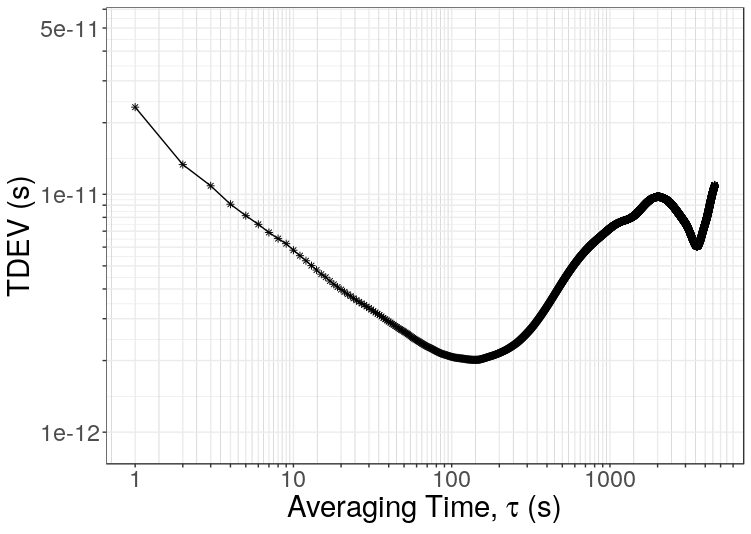
\includegraphics[width=0.7\linewidth]{img/tdev_exp3}
	\caption[TDEV of the end-nodes in the scalability test.]{Time Deviation 
	plot comparing the PPS signal from the end-nodes (WR-ZEN) to the Grand 
	Master of the network.}
	\label{fig:tdevnet}
\end{figure}

TDEV and MTIE values have been calculated by octaves, the numerical 
values can be found in Table \ref{tab:netresults}. For the short-therm 
stability we obtained a TDEV result of 2.32e-11 s. The minimum is reached at 
$\tau=64$, after that, frequency drift is observed from $\tau=200$ to 
$\tau=1000$ (see Figure \ref{fig:tdevnet}). The MTIE results show that maximum 
PPS error, during this test, is bounded below 2e-10 s (see Figure 
\ref{fig:mtienet}).

\begin{table*}\centering
	\ra{0.8}
	\begin{tabular}{@{} rcc@{}}%\toprule
		& TDEV (s)  & MTIE (s) \\ \midrule
		\textbf{$\tau$ (s)}\\
		\small{1}     & 2.32e-11  & 1.36e-10 \\
		%\small{2}     & 1.33315382e-11  & 1.36718750e-10 \\
		%\small{4}     & 9.08699704e-12  & 1.36718750e-10 \\
		\small{8}     & 6.51e-12  & 1.36e-10 \\
		%\small{16}    & 4.48330572e-12  & 1.36718750e-10 \\
		%\small{32}    & 3.22792513e-12  & 1.36718750e-10 \\
		\small{64}    & 2.37e-12  & 1.46e-10 \\
		%\small{128}   & 2.02186966e-12  & 1.46484375e-10 \\
		%\small{256}   & 2.36616321e-12  & 1.46484375e-10 \\
		\small{512}   & 4.38e-12  & 1.61e-10 \\
		\small{1024}  & 7.27e-12  & 1.66e-10 \\
		\small{2048}  & 9.75e-12  & 1.75e-10 \\
		\small{4096}  & 7.97e-12  & 1.90e-10 \\
		%\small{8192}  &                 & 2.00195313e-10 \\
		
		\bottomrule
	\end{tabular}
	\caption{This table contains the Time Deviation and Maximum Time Interval 
	Error results from the scalability test.}
	\label{tab:netresults}
\end{table*}

With those findings, it has been proved that a WR network with two levels can 
provide synchronization to all the equipment expected for the SKA facilities. 
It is also important to mention that some links could be broken in two WR links 
due to distance to some antennas, e.g. an intermediate WR device will be placed 
between the master WRS and the end-node. Introducing an extra WR level for some 
antennas should not be a problem to fulfil the timing requirements, a prove of 
that can be found in \cite{torres2016scalability}, where the results show that 
even a 10-hop network can reach the required time-budget for SKA.

Although long-distance fibre links have been used for that test, thermal 
influence should be considered previous to confirm the goodness of the 
WR solution for the SKA's timing distribution system. 

\begin{figure}
	\centering
	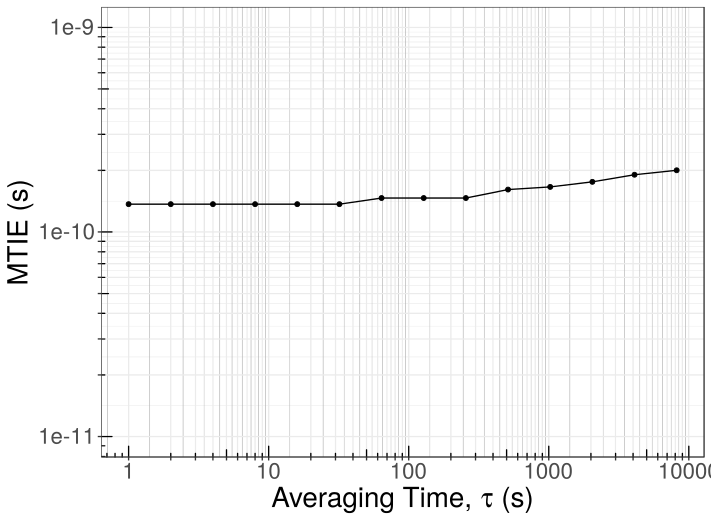
\includegraphics[width=0.7\linewidth]{img/mtie_exp3}
	\caption[MTIE of the end-nodes in the scalability test.]{Maximum Time 
	Interval Errorplot comparing the PPS signal from the end-nodes (WR-ZEN) to 
	the Grand Master of the network.}
	\label{fig:mtienet}
\end{figure}

\subsection{Temperature influence on time accuracy}
%\subsection{Fibre operational temperature influence on time accuracy}
\label{subsec:temp}

One of the key aspects of the timing solution for the SKA facilities is the 
influence evaluation of the external elements in the timing performance. 
Synchronization signals are spread over hundred of nodes which are connected by 
long distance fibre links. Meteorological elements, such as wind or large 
temperature changes, can alter propagation delays over the fibre 
links. The timing solution must compensate appropriately those effects in order 
to maintain the synchronization performance inside the limits required by the 
SKA's infrastructure. 

The proposed system has been tested by JIVE in the SKA specific dessert zones of 
the South Africa and \cite{paul-boven-paper-icalepcs} describes the main issues 
that must be taken into consideration. The main conclusion of this study is the
need of compensation techniques in order to control the timing drift due to
temperature changes.

In this contribution, we have focused on the temperature change effect over the 
cable
\textit{round-trip} time (CRTT) and the PPS performance. To evaluate that, we 
have used a climate chamber in the laboratory and some fibre spools of tens of 
kilometers. Wind impact has not been evaluated properly with our equipment, 
because of this, the experiments will only determine temperature effect on 
synchronization.

Theoretically, WR is able to dynamically calibrate the master to slave 
propagation delay from the total \textit{round-trip} time, and therefore PPS 
offset shall maintain constant even when the propagation delay changes. The 
accurate estimation of the one-way propagation delay is achieved by the use of 
a constant value, $\alpha$, which express the ratio between propagation times 
with the two wavelengths used in the WR link. A complete explanation of the 
link model could be read in \cite{Wlostowski2011} and \cite{Daniluk2012}.

In the real world, $\alpha$ is temperature dependent, because of the change in 
the refraction index due to a temperature variation in the fibre. For small and 
mid-distance links, in laboratory conditions, $\alpha$ is nearly negligible and 
the current link model behaves very well. The WR network in SKA will be formed 
by long distance links exposed to external elements. 

%In the concrete situation of the South Africa facilities, the chosen location 
% was the Karoo region. This region is a semi-desert area, very adequate to reduce human interferences in the high resolution data acquisition equipment, but with a inconvenient 
%respect to the temperature point of view: desert zones have a high difference 
%between day and night temperatures.

\begin{figure}
	\centering
	\includegraphics[width=0.7\linewidth]{img/tempsetup}
	\caption[Configuration of the climate chamber experiments]{Experimental 
		setup to analyse the influence of the temperature gradient over the 
		fibre link and the synchronization accuracy.}
	\label{fig:tempsetup}
\end{figure}

We performed a series of experiments introducing a 50 km length fibre spool in 
a climate chamber. The CRTT and the PPS offset between master and slave have 
been measured for a temperature range from 20 ºC to 50 ºC with 10 ºC steps. 

\begin{table*}\centering
	\ra{0.8}
	\begin{tabular}{@{} cccccc@{}}%\toprule
		& \multicolumn{2}{c}{\bfseries{RTT (ps)}} & &
		\multicolumn{2}{c}{\bfseries{PPS $offset_{SM}$ (ps)}} \\
		\cmidrule(l){2-3}  \cmidrule{5-6}
		\textbf{Spool temp (ºC)} & $\overline{x}$ & $s$ & & $\overline{x}$ 
		& $s$ \\ \midrule
		\small{20} & 478471695 & 303 & & 193 & 17 \\
		\small{30} & 478503719 & 50  & & 203 & 17 \\
		\small{40} & 478533492 & 807 & & 150 & 17 \\
		\small{50} & 478567050 & 399 & & 110 & 14 \\
		\bottomrule
	\end{tabular}
	\caption{Results of the thermal characterization for an operational fibre 
		temperature in range 20ºC to 50ºC with 10ºC steps.}
	\label{tab:temp}
\end{table*}

Our test is intended to prove the hypothesis that PPS offset is not related to 
the cable \textit{round-trip} time, i.e. changes in CRTT will not affect the 
synchronization accuracy. We have performed a series of experiments where the 
operational temperature of a 50 km fibre link is set in a point from 20ºC to 
50ºC. When the fibre reached the target temperature, we started to measure the 
rest of dependent values such as CRTT and PPS offset. All the WR equipment was 
calibrated in order to compensate the characteristic delays of each device 
following the official calibration procedure \cite{man:calib}.  The test setup 
is depicted in figure \ref{fig:tempsetup}.

The most relevant results are included in Table \ref{tab:temp}: (i) the mean 
value of CRTT and PPS offset samples, and (ii) their sample standard deviation. 
A total of 7200 samples (2 hours) per temperature step have been used to 
compute the presented statistics. The amplitude of the CRTT sampled data is 
96496 ps. Dividing it by the temperature range we obtained a CRTT variation of 
3213 ps/ºC. It is important to remark the huge change in the propagation delay. 
Considering a synchronization system that is not capable of dynamically 
calibrate that change, the final performance would suffer of an enormous 
degradation, which is unacceptable for the SKA equipment. The peak-to-peak 
difference for the PPS offset is 211 ps which leaves us a 7 ps/ºC and if we 
divide by the total link length: $0.14 ps/ºC \cdot km$.

%\begin{figure}
%	\centering
%	\begin{subfigure}[t]{0.48\textwidth}
%		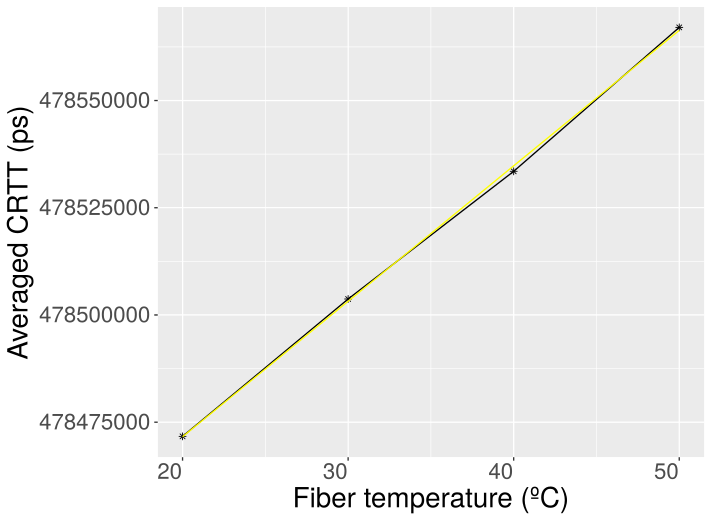
\includegraphics[width=\textwidth]{img/crttvstemp}
%		\caption[CRTT vs. Fiber temperature]{The figure shows the relation 
%			between the fibre temperature and the cable round-trip time.}
%		\label{fig:crttvstemp}
%	\end{subfigure}
%	~ % This symbol adds a white space between images
%	\begin{subfigure}[t]{0.48\textwidth}
%		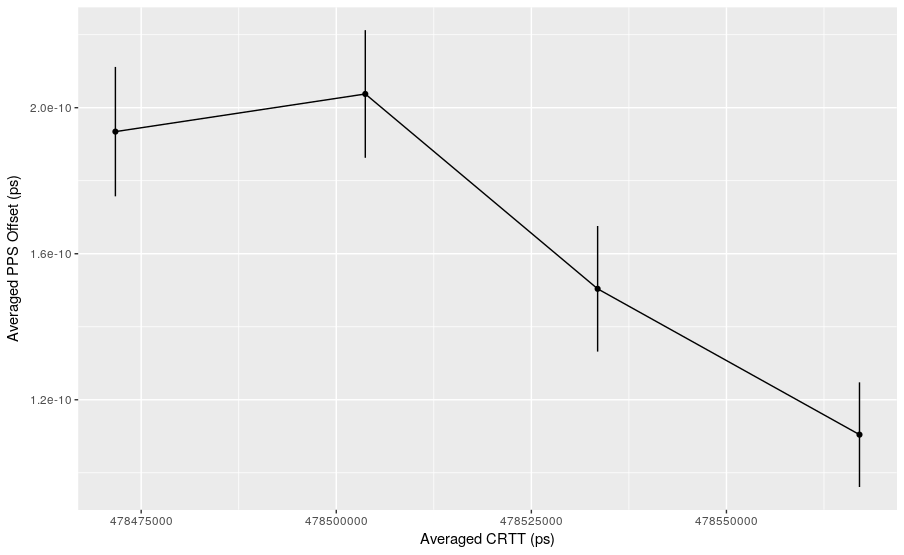
\includegraphics[width=\textwidth]{img/ppsvscrtt}
%		\caption[PPS offset vs. CRTT]{This figure shows how PPS offset is 
%			sightly influenced by changes in the cable round-trip time.}
%		\label{fig:ppsvscrtt}
%	\end{subfigure}
%	\caption{Evaluation of the cable \textit{round-trip} time and the PPS 
%		offset with variable temperature conditions for the fibre link.}
%\end{figure}


	
\begin{figure}[t]
	\centering
	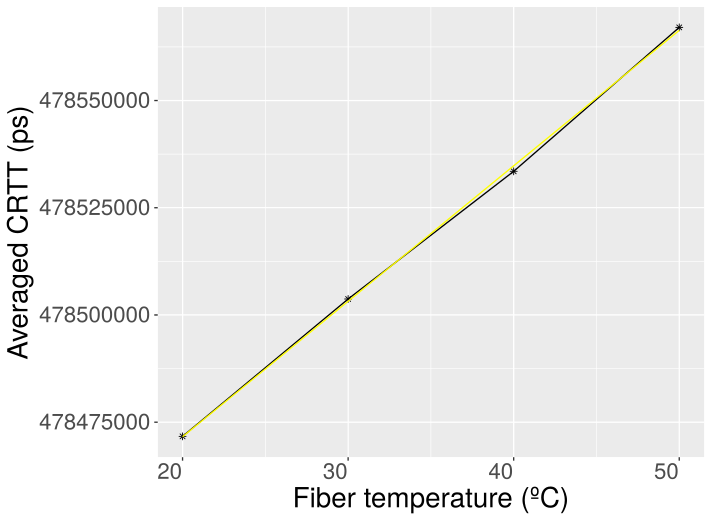
\includegraphics[width=0.7\linewidth]{img/crttvstemp}
	\caption[CRTT vs. Fiber temperature]{The figure shows the relation 
	between the fibre temperature and the cable round-trip time.}
	\label{fig:crttvstemp}
\end{figure}

\begin{figure}[t]
	\centering
	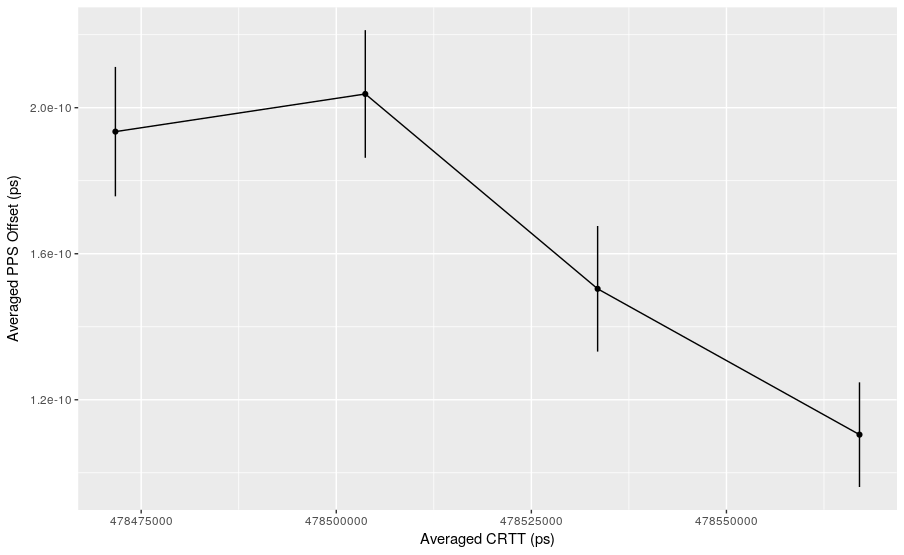
\includegraphics[width=0.7\linewidth]{img/ppsvscrtt}
	\caption[PPS offset vs. CRTT]{This figure shows how PPS offset is 
	sightly influenced by changes in the cable round-trip time.}
	\label{fig:ppsvscrtt}
	\caption{Evaluation of the cable \textit{round-trip} time and the PPS 
	offset with variable temperature conditions for the fibre link.}
\end{figure}

Figure \ref{fig:crttvstemp} shows a clear linear dependency between the 
temperature and the CRTT. Although, the PPS offset is not constant as 
we suppose in our initial hypothesis. The Figure \ref{fig:ppsvscrtt} suggests 
an inverse linear dependency between CRTT and offset, but if we take the 
standard error values into account, we can not state clearly that linear 
relation. It must be considered that $\alpha$ is computed experimentally using 
fixed-point arithmetic (the LM32 has no floating-point unit). While it seemed 
to work right for distances lower than a few kilometres, it may be insufficient 
for such long distances as we used in our experiments. Nevertheless, the 
observed offset variation for a long distance link and a 30ºC temperature 
gradient is only 200 ps that joined to the results from the previous 
experiments make the new PPS distribution system suitable for the SKA 
timing system.